\chapter{iMote2 Hardware}
For this thesis the Imote2 hardware platform was used. The Imote2 platform
consists of different pluggable boards to extend it with sensoric or multimedia
capabilities. For our work we only used the Imote2 Processor Radio board
(IPR2400) and the Interface Board (IIB2400) for serial console access and JTAG.

While other sensor nodes are tightly constrained regarding their computing power
and storage the Imote2 is based on a powerful XScale CPU and equipped with 32
MByte of SDRAM and flash storage. This comes of course with a higher power
consumption cost compared to microcontroller based sensor nodes like the T-Mote
Sky. On the other hand exactly these components are allowing us to run a full
Linux and DTN system on the node and allow comfortable development.

\section{Processor Radio Board}
As the name suggests this is the base board all other boards rely on. It holds
the PXA271 XScale ARM System on a Chip with a cpu frequency from 13 to 416 MHz
as well as the 32 MB SDRAM and the 32 MB flash storage. If configured for a
frequency from 13 to 104 MHz the CPU can be used in a low power mode on a low
voltage level (0.85V). This was not done during this work, but would be an
interesting target for real deployment.

The PXA271 offers a wide range of periphery components already build in. The
connections for this are available on the basic and advanced connectors on the
board. Examples would be USB host and client, SDIO, UART, AC97 and I2S audio
interfaces, I2C, SPI and GPIOs. USB client is already routed to a mini USB
connector on the board. This can be used to access the system as well as supply
power over USB.

The only other component that is directly build onto this board is the 802.15.4
radio plus antenna. We go into more details about it in the next section.

\begin{figure}
  \begin{center}
    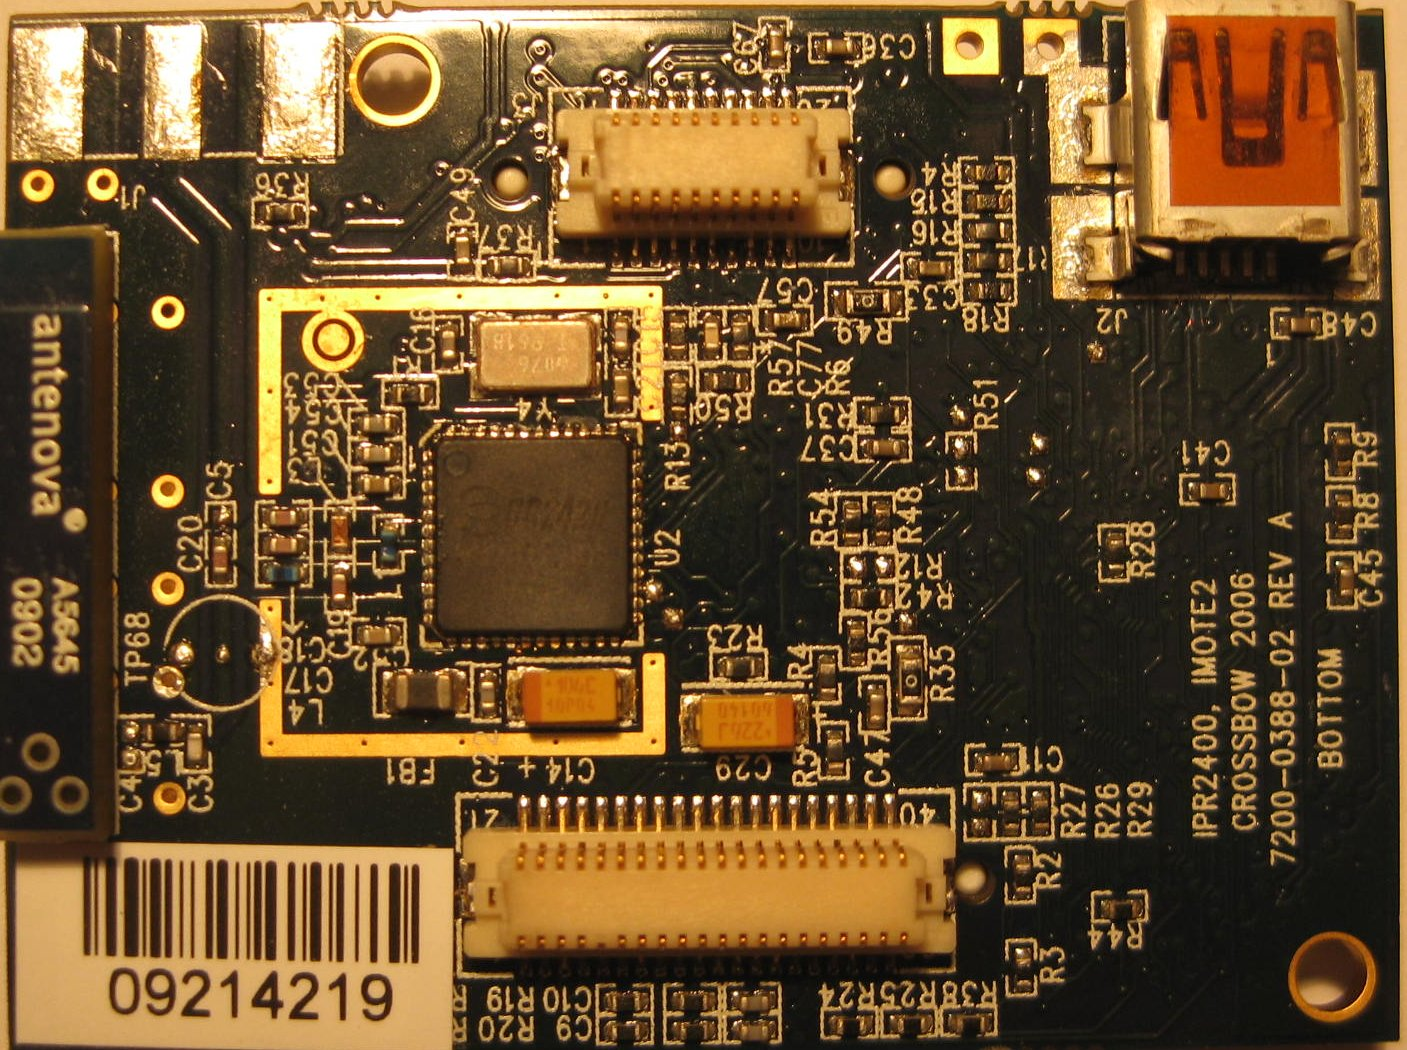
\includegraphics[height=6cm]{images/imote_top_cutted}
    \caption{Top side of the Processor Radio Board with the CC2420 and its antenna}
        \label{fig:imote2top}
  \end{center}
\end{figure}

\section{CC2420 802.15.4 Transceiver}
The used 802.15.4 radio on the Imote2 is a CC2420 from ChipCon nowadays TI.
Configuration and data transfer is done over SPI while some extra signalling
GPIOs are used for interrupts when the data FIFO is full, a complete package
arrived or a start frame delimiter (SFD) was recognized.

The CC2420 is a full-function device (FFD) and as such can be used as
coordinator or normal node. It only uses the 2.4 GHz band out of the three
available bands. It supports all sixteen channels on this band. Channel 11
(2.405 GHz) to 26 (2.480 GHz). It also supports the highest data rate available
in 802.15.4 with 250 kb/s. Configuration modes for the radio transmission power
are available to either save power or extend range.

More hardware support is available for CRC checking, data encryption, clear
channel assignment, auto acknowledge, link quality indication and more. While
the lack of support for all frequency bands is a pity the extended hardware
enabled functionality plus the easy to use SPI interface makes the chip a good
choice.
